\documentclass[landscape,final,a0paper,fontscale=0.285]{baposter}

\usepackage{calc}
\usepackage{graphicx}
\usepackage{amsmath}
\usepackage{amssymb}
\usepackage{relsize}
\usepackage{multirow}
\usepackage{rotating}
\usepackage{bm}
\usepackage{url}
\usepackage{xcolor}

\usepackage{graphicx}
\usepackage{multicol}

%\usepackage{times}
%\usepackage{helvet}
%\usepackage{bookman}
\usepackage{palatino}

% \usepackage{graphicx}
% \usepackage{draftwatermark}
% \SetWatermarkLightness{0.9}
% \SetWatermarkText{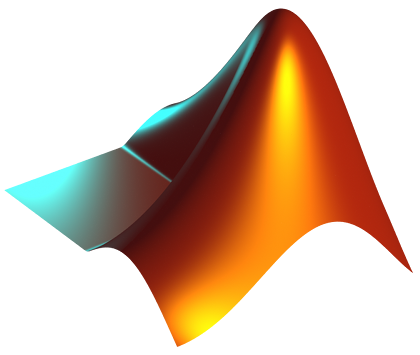
\includegraphics[angle=-45]{mlogs_cropped.png}}

% \usepackage{background}
% \backgroundsetup{contents={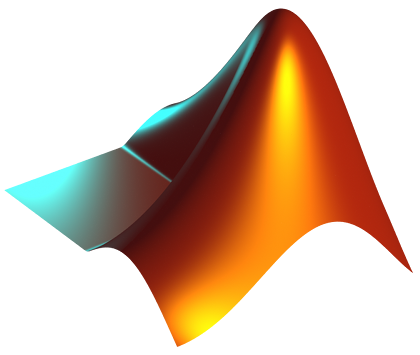
\includegraphics[scale=0.4]{mlogs_cropped.png}}}

\newcommand{\captionfont}{\footnotesize}

\graphicspath{{images/}{../images/}}
\usetikzlibrary{calc}

\newcommand{\SET}[1]  {\ensuremath{\mathcal{#1}}}
\newcommand{\MAT}[1]  {\ensuremath{\boldsymbol{#1}}}
\newcommand{\VEC}[1]  {\ensuremath{\boldsymbol{#1}}}
\newcommand{\Video}{\SET{V}}
\newcommand{\video}{\VEC{f}}
\newcommand{\track}{x}
\newcommand{\Track}{\SET T}
\newcommand{\LMs}{\SET L}
\newcommand{\lm}{l}
\newcommand{\PosE}{\SET P}
\newcommand{\posE}{\VEC p}
\newcommand{\negE}{\VEC n}
\newcommand{\NegE}{\SET N}
\newcommand{\Occluded}{\SET O}
\newcommand{\occluded}{o}

%%% change tiff to png
\usepackage{epstopdf}
\epstopdfDeclareGraphicsRule{.tif}{png}{.png}{convert #1 \OutputFile}
\AppendGraphicsExtensions{.tif}

%%% change bullet points to triangles
\usepackage{amssymb}
\renewcommand{\labelitemi}{$\blacktriangleright$}

%% for plus minus sign
\usepackage{mathpazo}

% We therefore load the caption package which provides
% the command \captionof
% Set up how figure and table captions are displayed
\usepackage{caption}
\captionsetup{
  font=small,% set font size to footnotesize
  labelfont=bf % bold label (e.g., Figure 3.2) font
}


%%% for references
\usepackage{biblatex}

\usepackage{filecontents}
\usepackage[T1]{fontenc}
\usepackage[utf8]{inputenc}
\usepackage{geometry}
\geometry{textwidth=7cm}

\usepackage{etoolbox,fancyhdr}% http://ctan.org/pkg/{etoolbox,fancyhdr,xcolor}
% \patchcmd{<cmd>}{<search>}{<replace>}{<success>}{<failure>}
\newcommand{\headrulecolor}[1]{\patchcmd{\headrule}{\hrule}{\color{#1}\hrule}{}{}}
\newcommand{\footrulecolor}[1]{\patchcmd{\footrule}{\hrule}{\color{#1}\hrule}{}{}}
\pagestyle{fancy}
\fancyhf{}% Clear header/footer
 \fancyfoot[R]{\thepage}
\renewcommand{\headrulewidth}{0.4pt}% Default \headrulewidth is 0.4pt
\renewcommand{\footrulewidth}{0.4pt}% Default \footrulewidth is 0pt
\headrulecolor{red!70}% Set header rule colour to 70% red.
 
\usepackage{tgbonum}

\begin{filecontents}{\jobname.bib}

@misc{bworld,
  author = {Brian Shute},
  title = {{Overcoming The Hurdle Of Controlling Stoma Noise}},
  howpublished = "\url{http://www.drshute.com/archives/2004_08.html}",
  year = {2004}, 
  note = "[Online; accessed 21-October-2017]"
}


@online{ErokyarAgeGender,
author = {Erokyar, Hasan.},
title = {Age and Gender Recognition for Speech Applications based on Support Vector Machines},
month = {January},
year = {2014},
%url = {http://scholarcommons.usf.edu/cgi/viewcontent.cgi?article=6552&context=etd},
%note = {Last accessed: 2017-07-22}
}



\end{filecontents}
\addbibresource{\jobname.bib}

%%%%%%%%%%%%%%%%%%%%%%%%%%%%%%%%%%%%%%%%%%%%%%%%%%%%%%%%%%%%%%%%%%%%%%%%%%%%%%%%
%%%% Some math symbols used in the text
%%%%%%%%%%%%%%%%%%%%%%%%%%%%%%%%%%%%%%%%%%%%%%%%%%%%%%%%%%%%%%%%%%%%%%%%%%%%%%%%

%%%%%%%%%%%%%%%%%%%%%%%%%%%%%%%%%%%%%%%%%%%%%%%%%%%%%%%%%%%%%%%%%%%%%%%%%%%%%%%%
% Multicol Settings
%%%%%%%%%%%%%%%%%%%%%%%%%%%%%%%%%%%%%%%%%%%%%%%%%%%%%%%%%%%%%%%%%%%%%%%%%%%%%%%%
\setlength{\columnsep}{1.5em}
\setlength{\columnseprule}{0mm}

%%%%%%%%%%%%%%%%%%%%%%%%%%%%%%%%%%%%%%%%%%%%%%%%%%%%%%%%%%%%%%%%%%%%%%%%%%%%%%%%
% Save space in lists. Use this after the opening of the list
%%%%%%%%%%%%%%%%%%%%%%%%%%%%%%%%%%%%%%%%%%%%%%%%%%%%%%%%%%%%%%%%%%%%%%%%%%%%%%%%
\newcommand{\compresslist}{%
\setlength{\itemsep}{1pt}%
\setlength{\parskip}{0pt}%
\setlength{\parsep}{0pt}%
}

%%%%%%%%%%%%%%%%%%%%%%%%%%%%%%%%%%%%%%%%%%%%%%%%%%%%%%%%%%%%%%%%%%%%%%%%%%%%%%
%%% Begin of Document
%%%%%%%%%%%%%%%%%%%%%%%%%%%%%%%%%%%%%%%%%%%%%%%%%%%%%%%%%%%%%%%%%%%%%%%%%%%%%%

\begin{document}

%%%%%%%%%%%%%%%%%%%%%%%%%%%%%%%%%%%%%%%%%%%%%%%%%%%%%%%%%%%%%%%%%%%%%%%%%%%%%%
%%% Here starts the poster
%%%---------------------------------------------------------------------------
%%% Format it to your taste with the options
%%%%%%%%%%%%%%%%%%%%%%%%%%%%%%%%%%%%%%%%%%%%%%%%%%%%%%%%%%%%%%%%%%%%%%%%%%%%%%
% Define some colors

%\definecolor{lightblue}{cmyk}{0.83,0.24,0,0.12}
\definecolor{lightblue}{rgb}{0.145,0.6666,1}
\definecolor{navyblue}{RGB}{2, 12, 28}
\definecolor{nn}{RGB}{0,0,27}
\definecolor{dd}{RGB}{255, 255, 105}%{0,0,53}
\definecolor{headerBlue}{RGB}{20,50,100}

\definecolor{blue(ryb)}{rgb}{0.01, 0.28, 1.0}
\definecolor{azure(colorwheel)}{rgb}{0.0, 0.5, 1.0}
\definecolor{blue(pigment)}{rgb}{0.2, 0.2, 0.6}
\definecolor{cobalt}{rgb}{0.0, 0.28, 0.67}



\hyphenation{resolution occlusions}
%%
\begin{poster}%
  % Poster Options
  {
  % Show grid to help with alignment
  grid=false,
  % Column spacing
  colspacing=1em,
  % Color style
  bgColorOne=white,
  bgColorTwo=white,
  borderColor=cobalt,
  headerColorOne=cobalt,
  headerColorTwo=lightblue,
  headerFontColor=white,
  boxColorOne=white,
  boxColorTwo=lightblue,
  % Format of textbox
  textborder=rectangle,%roundedleft,
  % Format of text header
  eyecatcher=true,
  headerborder=closed,
  headerheight=0.1\textheight,
%  textfont=\sc, An example of changing the text font
  headershape=rounded,%roundedright,
  headershade=shadelr,
  headerfont=\Large\bf\textsc, %Sans Serif
  textfont={\setlength{\parindent}{1.5em}},
  boxshade=plain,
%  background=shade-tb,
  background=plain,
  linewidth=2pt
  }
  % Eye Catcher
  { 
\includegraphics[height=6.5em]{wits.jpg}} 
  %
\includegraphics[height=6.5em,width=12em]{f.png}
  % Title
  { \textcolor{headerBlue}{\fontfamily{lmss}\selectfont LISTEN \hspace{1mm}TO\hspace{1mm}  YOUR \hspace{1mm} HEART}\vspace{0.25em}}
  % Authors
  {\fontfamily{lmss}\selectfont Boikanyo Radiokana (1386807) \& Elias Sepuru (1427726)\\ Supervisor - Ellen De Mello Koch }
  % University logo
  {% The makebox allows the title to flow into the logo, this is a hack because of the L shaped logo.
    
\includegraphics[height=6.5em]{EIE-Logo-Full-Colour.png}
  }

%%%%%%%%%%%%%%%%%%%%%%%%%%%%%%%%%%%%%%%%%%%%%%%%%%%%%%%%%%%%%%%%%%%%%%%%%%%%%%
%%% Now define the boxes that make up the poster
%%%---------------------------------------------------------------------------
%%% Each box has a name and can be placed absolutely or relatively.
%%% The only inconvenience is that you can only specify a relative position 
%%% towards an already declared box. So if you have a box attached to the 
%%% bottom, one to the top and a third one which should be in between, you 
%%% have to specify the top and bottom boxes before you specify the middle 
%%% box.
%%%%%%%%%%%%%%%%%%%%%%%%%%%%%%%%%%%%%%%%%%%%%%%%%%%%%%%%%%%%%%%%%%%%%%%%%%%%%%
    %
    % A coloured circle useful as a bullet with an adjustably strong filling
    \newcommand{\colouredcircle}{%
      \tikz{\useasboundingbox (-0.2em,-0.32em) rectangle(0.2em,0.32em); \draw[draw=black,fill=lightblue,line width=0.03em] (0,0) circle(0.18em);}}

%%%%%%%%%%%%%%%%%%%%%%%%%%%%%%%%%%%%%%%%%%%%%%%%%%%%%%%%%%%%%%%%%%%%%%%%%%%%%%
  \headerbox{Introduction}{name=problem,column=0,row=0}{
%%%%%%%%%%%%%%%%%%%%%%%%%%%%%%%%%%%%%%%%%%%%%%%%%%%%%%%%%%%%%%%%%%%%%%%%%%%%%%
   
   
  \begin{itemize}\compresslist
      \item According to WHO, Cardiovascular Diseases (CVD's) continue to be one of the leading causes of deaths globally.  
      \item To check for any CVD's (abnormalities) in patients' heartbeat sounds, medical practitioners currently use a method known as cardiac auscultation.
      \item This is a process whereby a medical practitioner listens to the heart sound, analyses it and classifies it as normal or abnormal.
      \item Generally it is a difficult skill to acquire considering the complexity of abnormal heart sounds.
      \item An easily accessible and reliable heartbeat sound classification system would be vital in reducing high mortality rates due to CVD's and also assist medical practitioners with more accurate cardiac auscultation.
  \end{itemize}
 
  \vspace{0.3em}
 }

%%%%%%%%%%%%%%%%%%%%%%%%%%%%%%%%%%%%%%%%%%%%%%%%%%%%%%%%%%%%%%%%%%%%%%%%%%%%%%
  \headerbox{Background Cont.}{name=contribution,column=1,row=0, span = 2}{
%%%%%%%%%%%%%%%%%%%%%%%%%%%%%%%%%%%%%%%%%%%%%%%%%%%%%%%%%%%%%%%%%%%%%%%%%%%%%%

   \begin{multicols}{2}
 % \setlength\abovecaptionskip{-15pt}
   \begin{centre}
 % \caption{A picture of the universe!}
  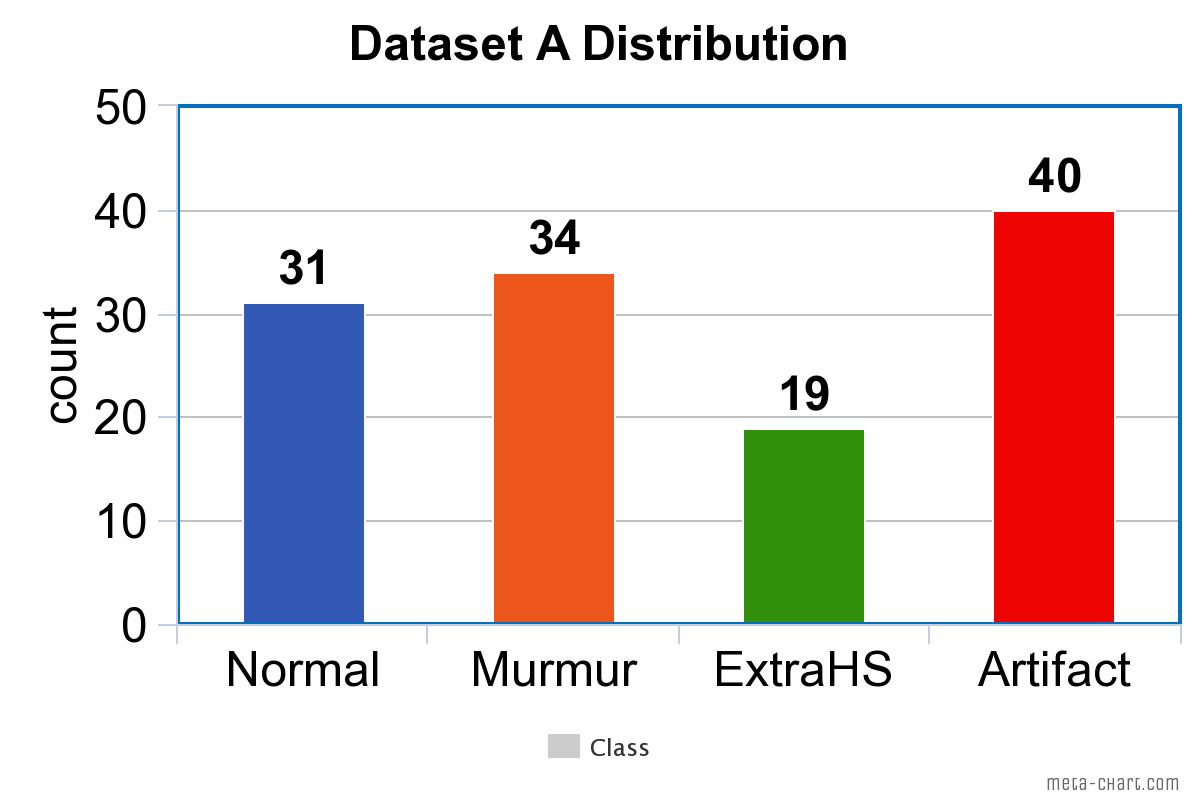
\includegraphics[height=9em, width = 4.5cm]{da.png}
   \captionof{figure}{Dataset A: iphone (iStethoscope)}%\cite{vlc1}}
  \end{centre}
   \vspace{0.3em}
   
    % \setlength\abovecaptionskip{-15pt}
   \begin{centre}
 % \caption{A picture of the universe!}
  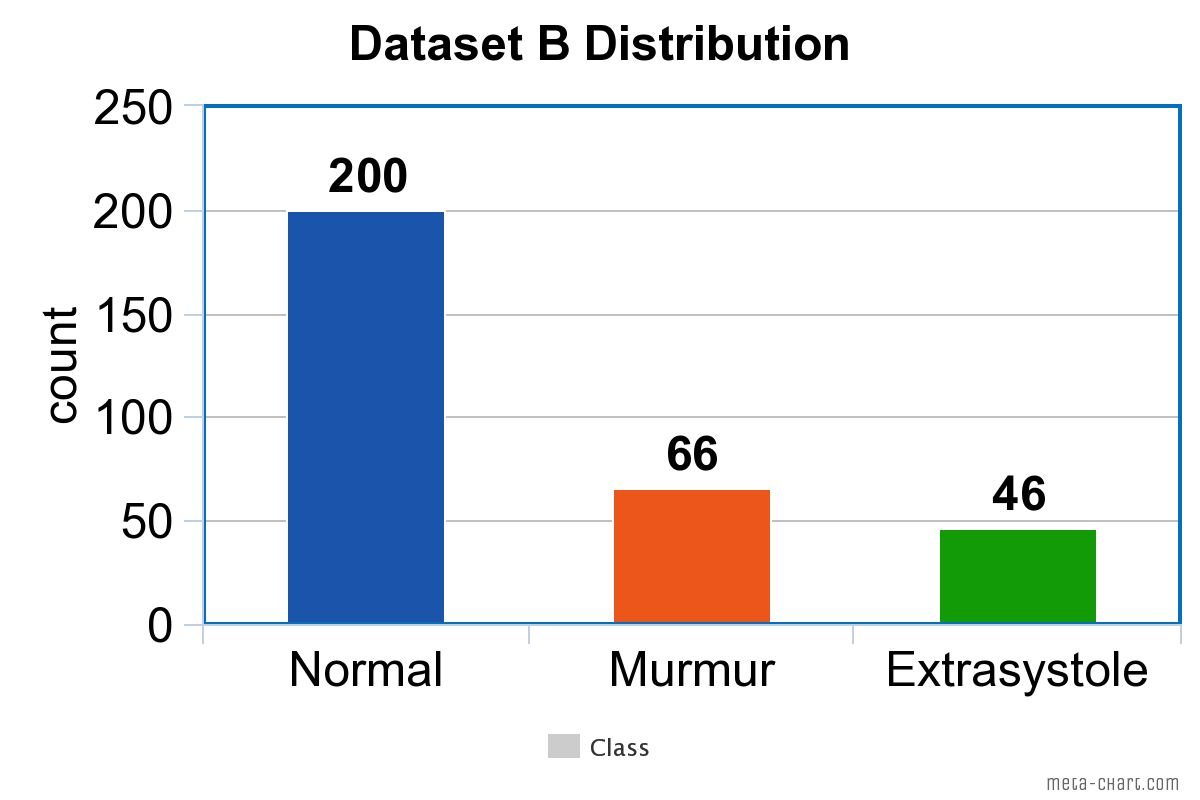
\includegraphics[height= 9em, width = 4.5cm]{db.png}
   \captionof{figure}{Dataset B: Digital stethoscope)}%\cite{vlc1}}
  \end{centre}
  \end{multicols}
%   \vspace{0.3em}
   
  
  }
  
%%%%%%%%%%%%%%%%%%%%%%%%%%%%%%%%%%%%%%%%%%%%%%%%%%%%%%%%%%%%%%%%%%%%%%%%%%%%%%
  \headerbox{Methodology}{name=background model,column=1,span = 2,below=contribution,bottomaligned=references}{
%%%%%%%%%%%%%%%%%%%%%%%%%%%%%%%%%%%%%%%%%%%%%%%%%%%%%%%%%%%%%%%%%%%%%%%%%%%%%%

  %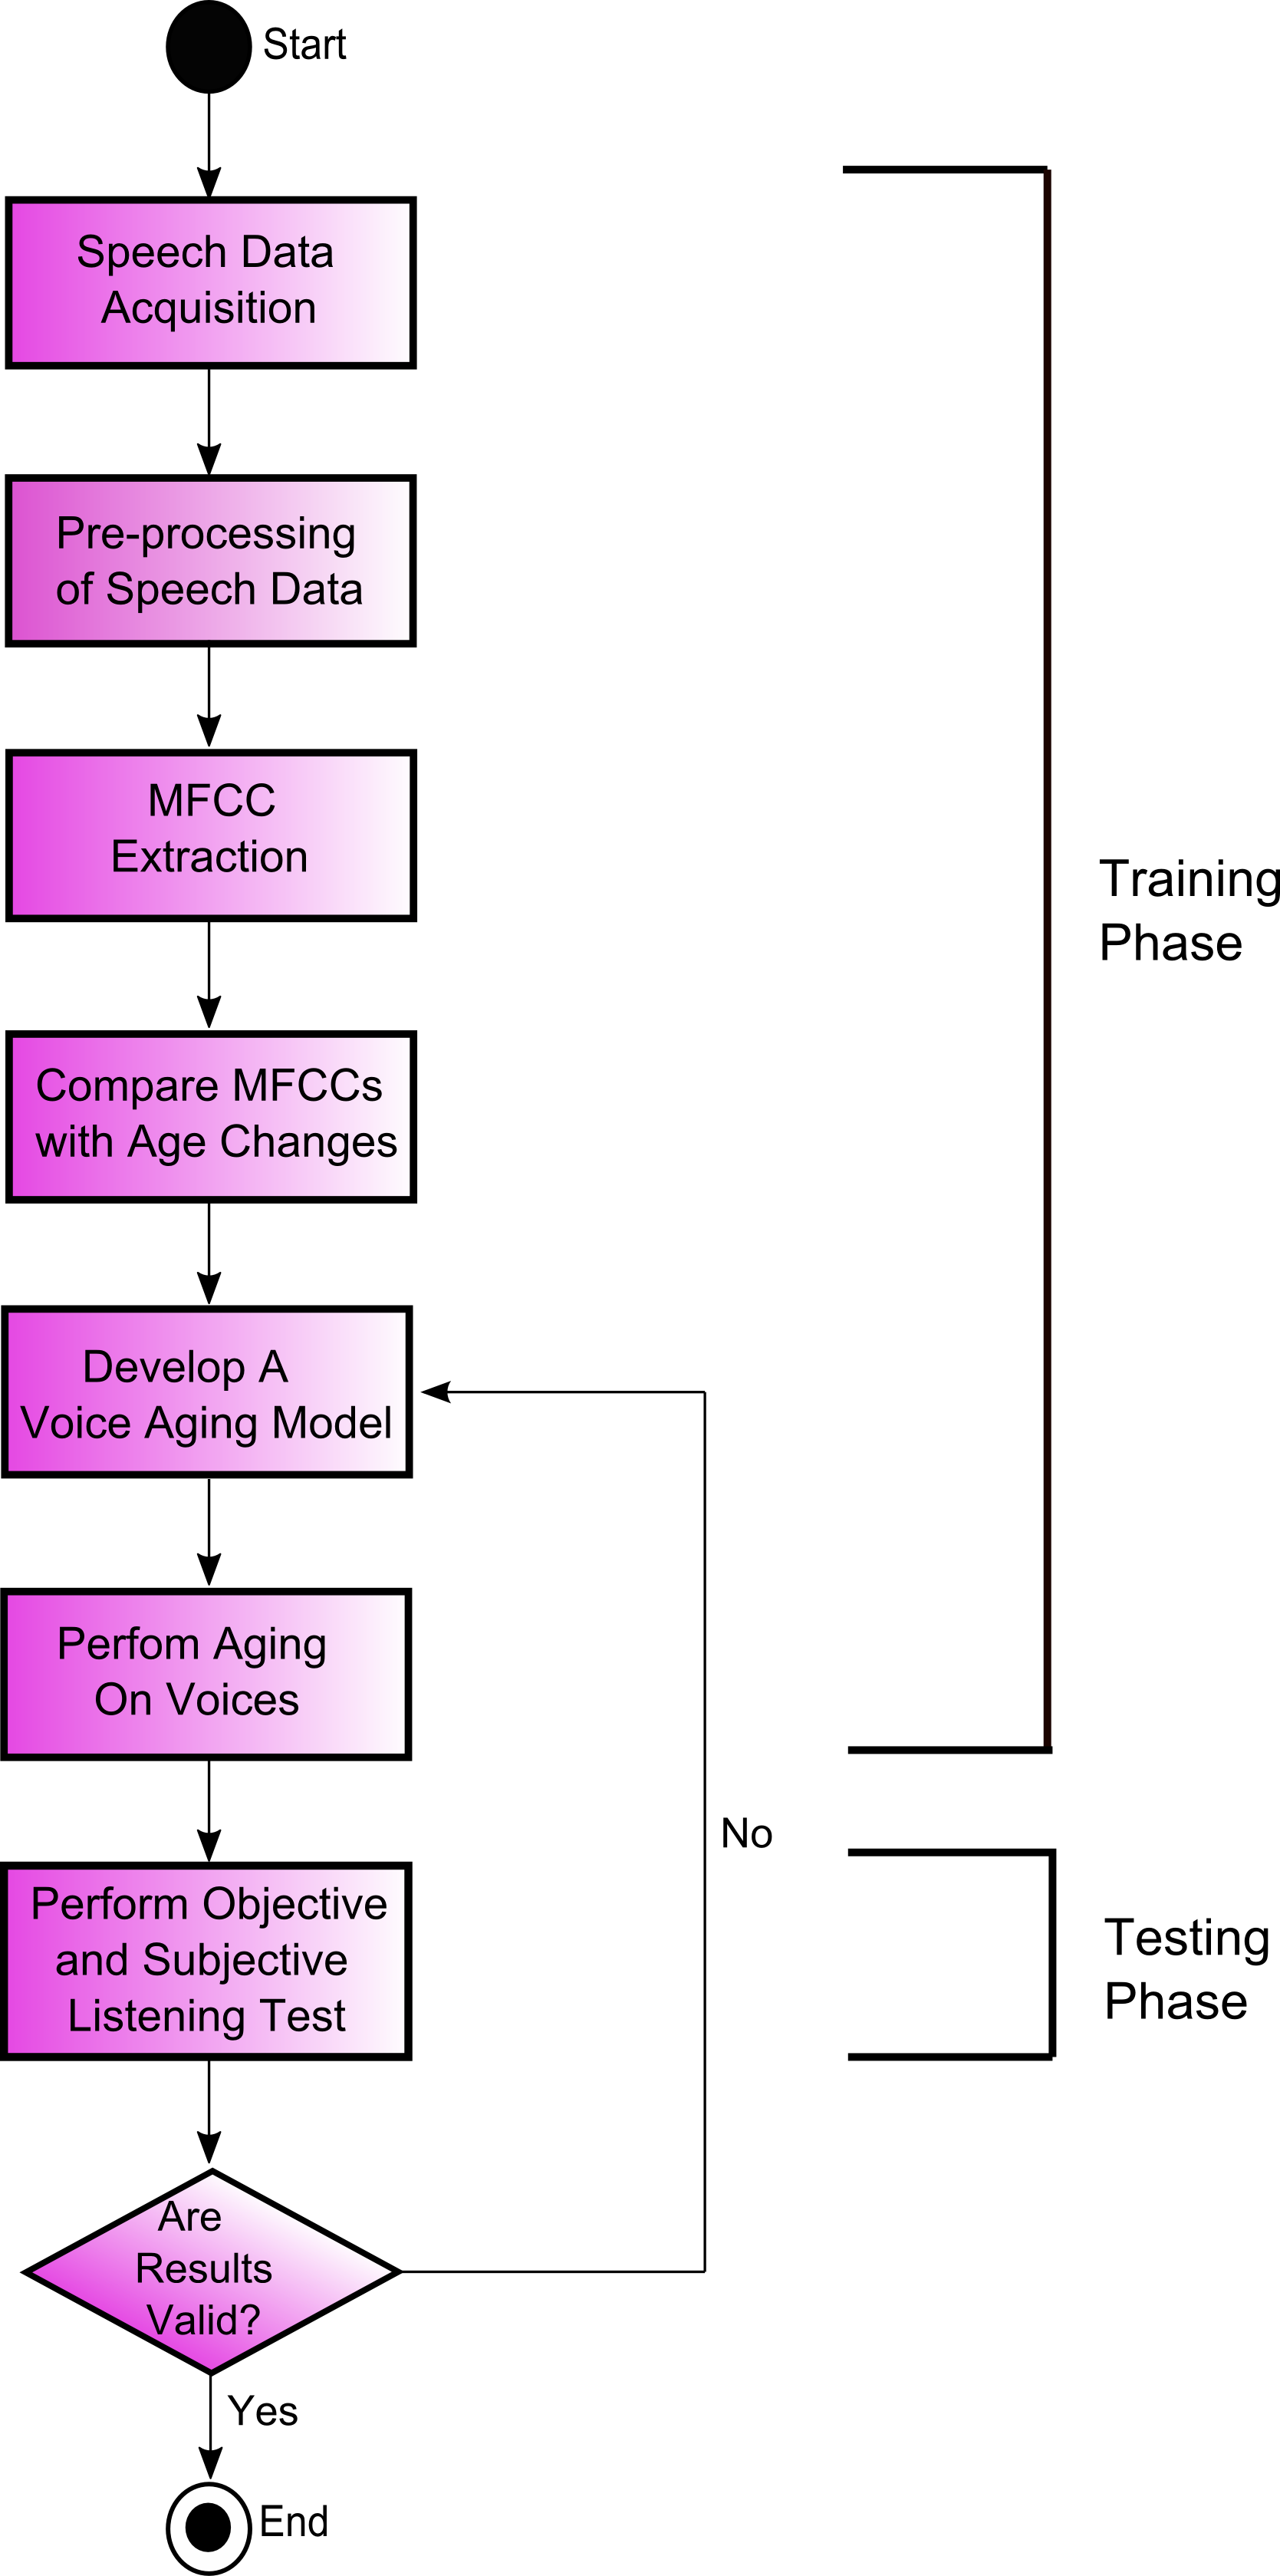
\includegraphics[height=35em]{algoVerticalNew.png}
  
  \begin{centre}
 % \caption{A picture of the universe!}
  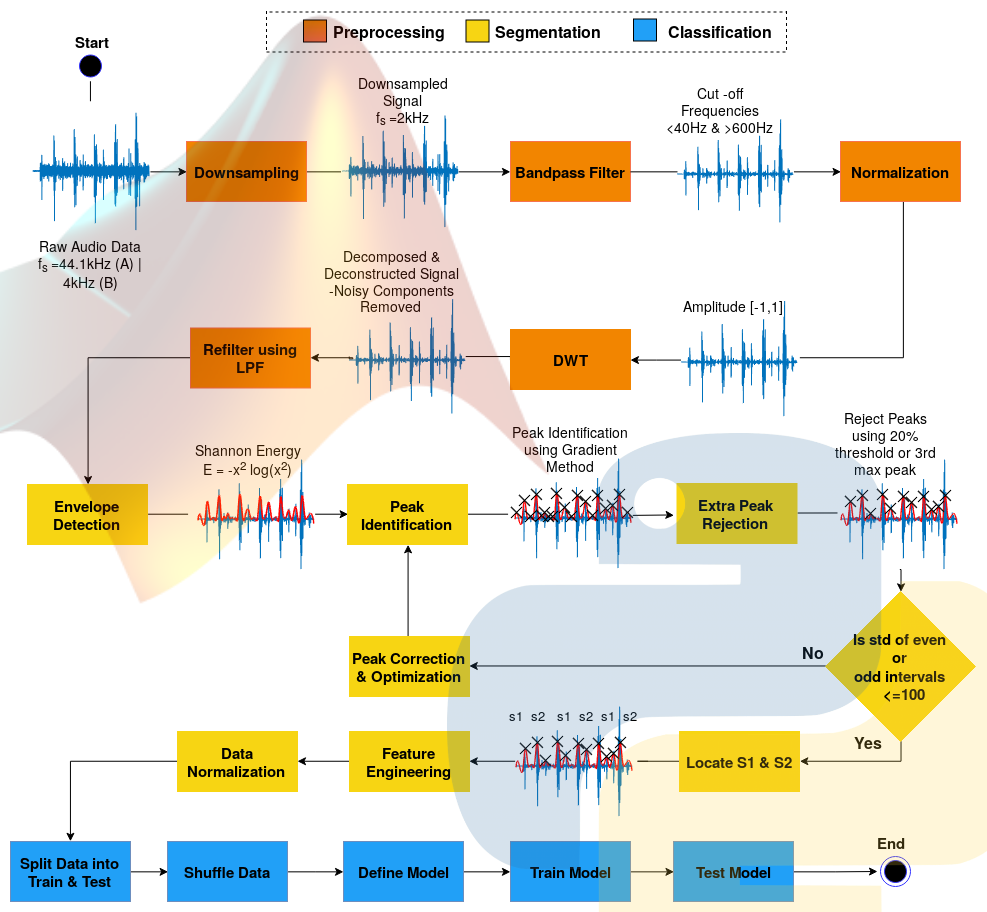
\includegraphics[scale = 0.43]{finalflowC1.png}
  \captionof{figure}{System Overview}%\cite{vlc1}}
  \end{centre}
  \vspace{0.3em}



  }


%%%%%%%%%%%%%%%%%%%%%%%%%%%%%%%%%%%%%%%%%%%%%%%%%%%%%%%%%%%%%%%%%%%%%%%%%%%%%%
\headerbox{Results \& Discussion}{name=results,column=3,row=0}{
  %%%%%%%%%%%%%%%%%%%%%%%%%%%%%%%%%%%%%%%%%%%%%%%%%%%%%%%%%%%%%%%%%%%%%%%%%%%%%%
\begin{center}
       \centering
       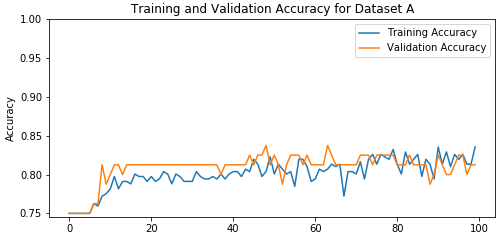
\includegraphics[height= 9em, width = 6cm]{validationA.png}
  \captionof{figure}{ANN performance (Dataset A)}%\cite{vlc1}}
  \end{center}{}

  \begin{center}
       \centering
       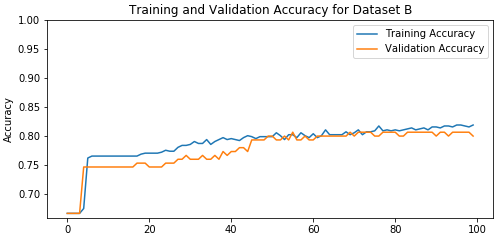
\includegraphics[height= 9em, width = 6cm]{Classification_B_80_81_No_Dropout_Validation_split.png}
  \captionof{figure}{ANN performance (Dataset B)}%\cite{vlc1}}
  \end{center}{}
  
  \begin{center}
       \centering
       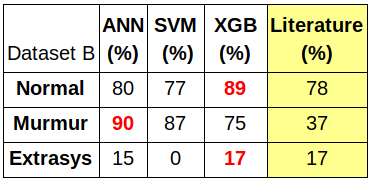
\includegraphics[height= 5.6em, width = 5.5cm]{table.png}
  \captionof{figure}{Performances for Dataset B}%\cite{vlc1}}
  \end{center}{}
  
  \begin{itemize}
      \item ANN performed best with high class precisions, however it was unable to classify Extrasystole heart sounds.
      \item This is due to a small training set used and Extrasystoles having similar characteristics to normal heart sounds.
  \end{itemize}{}
  
}
%%%%%%%%%%%%%%%%%%%%%%%%%%%%%%%%%%%%%%%%%%%%%%%%%%%%%%%%%%%%%%%%%%%%%%%%%%%%%%
  \headerbox{Background}{name=references,column=0,above=bottom}{
%%%%%%%%%%%%%%%%%%%%%%%%%%%%%%%%%%%%%%%%%%%%%%%%%%%%%%%%%%%%%%%%%%%%%%%%%%%%%%
  The dataset used is from a secondary source, collected from recordings using an iphone (iStethoscope app - Dataset A) and digital stethoscope (Dataset B). 
  

  \vspace{0.3em}
  }

%%%%%%%%%%%%%%%%%%%%%%%%%%%%%%%%%%%%%%%%%%%%%%%%%%%%%%%%%%%%%%%%%%%%%%%%%%%%%%
\headerbox{Conclusion}{name=speed,column=3,row=0,below=results}{
  %%%%%%%%%%%%%%%%%%%%%%%%%%%%%%%%%%%%%%%%%%%%%%%%%%%%%%%%%%%%%%%%%%%%%%%%%%%%%%
 
 ANN classifier was found to be the most promising audio heart sounds classifier. For future work, an equally distributed training set & distinct Extra-systole features are recommended.
    
   \vspace{0.0em}
  }
  
 
%%%%%%%%%%%%%%%%%%%%%%%%%%%%%%%%%%%%%%%%%%%%%%%%%%%%%%%%%%%%%%%%%%%%%%%%%%%%%%
  \headerbox{Project Objectives}{name=method,column=0,below=problem}{
%%%%%%%%%%%%%%%%%%%%%%%%%%%%%%%%%%%%%%%%%%%%%%%%%%%%%%%%%%%%%%%%%%%%%%%%%%%%%%
   \vspace{0.25em}
  
   \begin{itemize}%\compresslist
      \item To implement a method which can locate \textit{lub} and \textit{dub} sounds (S1 and S2) within audio data, segment the files and classify heartbeats into normal or diseased categories.
      \item To create a model that will enable a first level screening of detecting abnormalities in an individuals heart sound.
         \begin{itemize}
            \item For home use by individuals using a smartphone.
            \item For hospital use by medical professionals.
         \end{itemize}
    
   \end{itemize}
  
   \vspace{0.3em}
  }

  
%%%%%%%%%%%%%%%%%%%%%%%%%%%%%%%%%%%%%%%%%%%%%%%%%%%%%%%%%%%%%%%%%%%%%%%%%%%%%%
  \headerbox{Acknowledgements}{name=acknowledgements,column=3, above=bottom , below = speed}{
%%%%%%%%%%%%%%%%%%%%%%%%%%%%%%%%%%%%%%%%%%%%%%%%%%%%%%%%%%%%%%%%%%%%%%%%%%%%%%
 
  
  A special thanks to Ms Ellen De Mello Koch for her constant support and advice.

  }  

\end{poster}

\end{document}
